% Options for packages loaded elsewhere
\PassOptionsToPackage{unicode}{hyperref}
\PassOptionsToPackage{hyphens}{url}
%
\documentclass[
]{article}
\usepackage{lmodern}
\usepackage{amsmath}
\usepackage{ifxetex,ifluatex}
\ifnum 0\ifxetex 1\fi\ifluatex 1\fi=0 % if pdftex
  \usepackage[T1]{fontenc}
  \usepackage[utf8]{inputenc}
  \usepackage{textcomp} % provide euro and other symbols
  \usepackage{amssymb}
\else % if luatex or xetex
  \usepackage{unicode-math}
  \defaultfontfeatures{Scale=MatchLowercase}
  \defaultfontfeatures[\rmfamily]{Ligatures=TeX,Scale=1}
\fi
% Use upquote if available, for straight quotes in verbatim environments
\IfFileExists{upquote.sty}{\usepackage{upquote}}{}
\IfFileExists{microtype.sty}{% use microtype if available
  \usepackage[]{microtype}
  \UseMicrotypeSet[protrusion]{basicmath} % disable protrusion for tt fonts
}{}
\makeatletter
\@ifundefined{KOMAClassName}{% if non-KOMA class
  \IfFileExists{parskip.sty}{%
    \usepackage{parskip}
  }{% else
    \setlength{\parindent}{0pt}
    \setlength{\parskip}{6pt plus 2pt minus 1pt}}
}{% if KOMA class
  \KOMAoptions{parskip=half}}
\makeatother
\usepackage{xcolor}
\IfFileExists{xurl.sty}{\usepackage{xurl}}{} % add URL line breaks if available
\IfFileExists{bookmark.sty}{\usepackage{bookmark}}{\usepackage{hyperref}}
\hypersetup{
  pdftitle={DTC - Forecasting Home Price Index},
  pdfauthor={Eric Beekman, Jonathan Burns, Glen Lewis, and Andrew Nalundasan},
  hidelinks,
  pdfcreator={LaTeX via pandoc}}
\urlstyle{same} % disable monospaced font for URLs
\usepackage[margin=1in]{geometry}
\usepackage{graphicx}
\makeatletter
\def\maxwidth{\ifdim\Gin@nat@width>\linewidth\linewidth\else\Gin@nat@width\fi}
\def\maxheight{\ifdim\Gin@nat@height>\textheight\textheight\else\Gin@nat@height\fi}
\makeatother
% Scale images if necessary, so that they will not overflow the page
% margins by default, and it is still possible to overwrite the defaults
% using explicit options in \includegraphics[width, height, ...]{}
\setkeys{Gin}{width=\maxwidth,height=\maxheight,keepaspectratio}
% Set default figure placement to htbp
\makeatletter
\def\fps@figure{htbp}
\makeatother
\setlength{\emergencystretch}{3em} % prevent overfull lines
\providecommand{\tightlist}{%
  \setlength{\itemsep}{0pt}\setlength{\parskip}{0pt}}
\setcounter{secnumdepth}{-\maxdimen} % remove section numbering
\ifluatex
  \usepackage{selnolig}  % disable illegal ligatures
\fi

\title{DTC - Forecasting Home Price Index}
\author{Eric Beekman, Jonathan Burns, Glen Lewis, and Andrew Nalundasan}
\date{}

\begin{document}
\maketitle

+Forecasting Housing Prices

Housing price growth has exploded in recent months and house prices in
general have increased from 1975 onward. It has become vital to lenders,
individuals, and government officials to monitor changes in house prices
over time to appropriately plan for home ownership and changes in
housing affordability at scale. We want to investigate how house prices
have changed in the last decade and compare pre-pandemic to
post-pandemic price changes.

+Research Question

How did the pandemic impact the behavior of the housing price index and
what is the appropriate scheme (fixed, recursive, or rolling) that will
help us best forecast the housing price index values after the pandemic?

+Data Description

We used the Freddie Mac House Price Index (FMPHI) available at
\url{http://www.freddiemac.com/research/indices/house-price-index.page}.

Per the Freddie Mac website ``the FMHPI provides a measure of typical
price inflation for houses within the United States. Values are
calculated monthly and released at the end of the following month. For
example, the FMHPI for March is published in late April.'' The data
includes seasonally and non-seasonally adjusted series which are
available at three different geographical levels (metropolitan, state,
and national)for each month going all the way back to January 1975.

For our forecasting analysis we split the data into an estimation set
(1975 through 2019) and a prediction set (January 2020 onward)

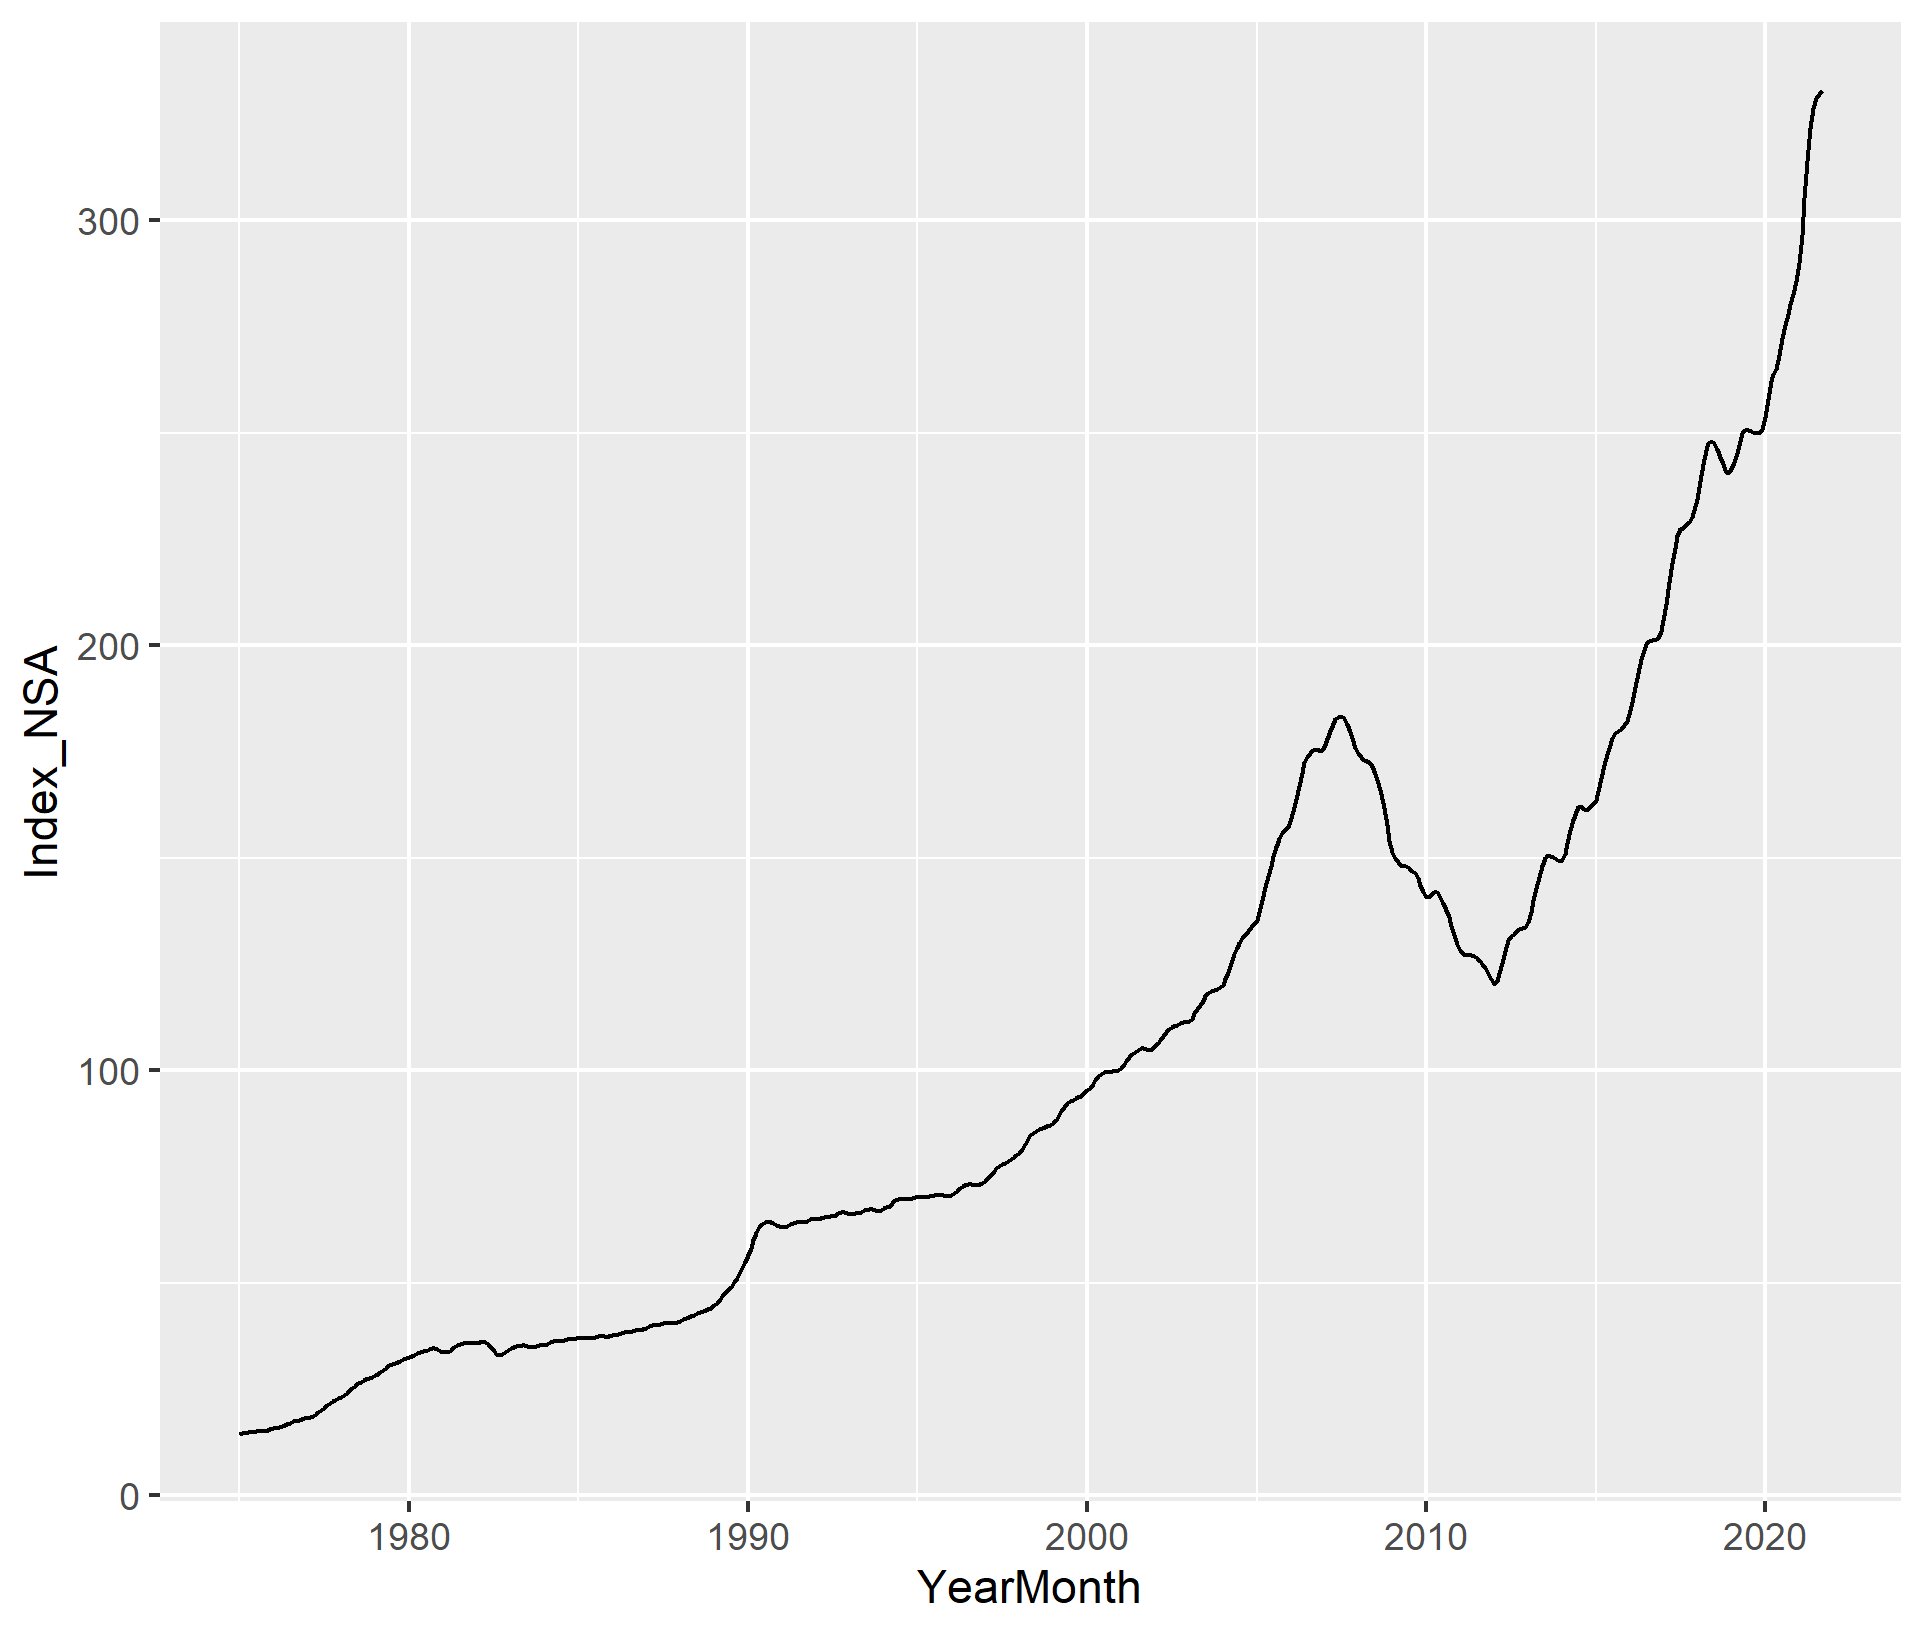
\includegraphics[width=5.20833in,height=5.20833in]{NSA-graph.png}

We have created the following ACFs and PACFs based on the estimate and
prediction sets of the data.

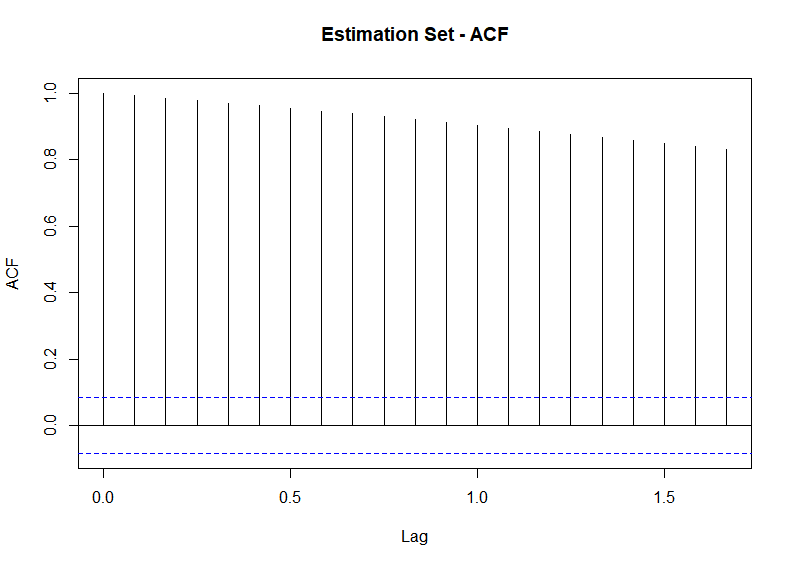
\includegraphics[width=5.20833in,height=5.20833in]{03_visuals/est_acf.png}

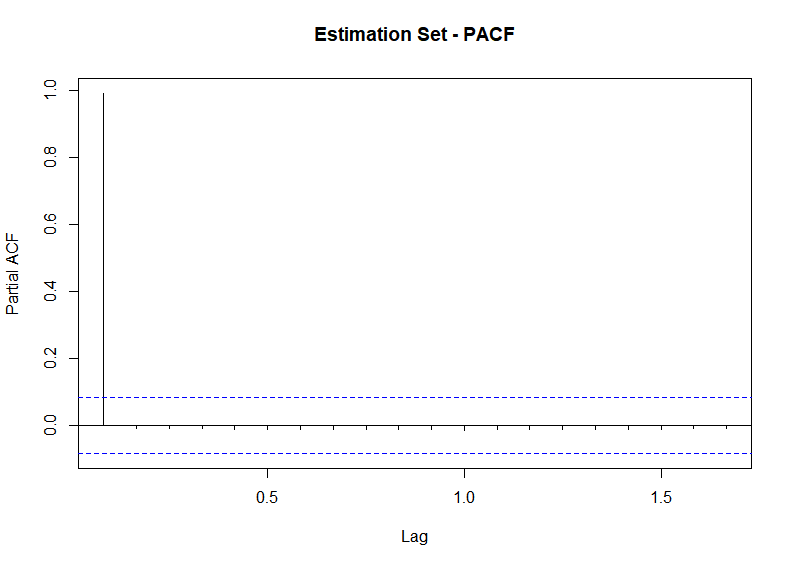
\includegraphics[width=5.20833in,height=5.20833in]{03_visuals/est_pacf.png}

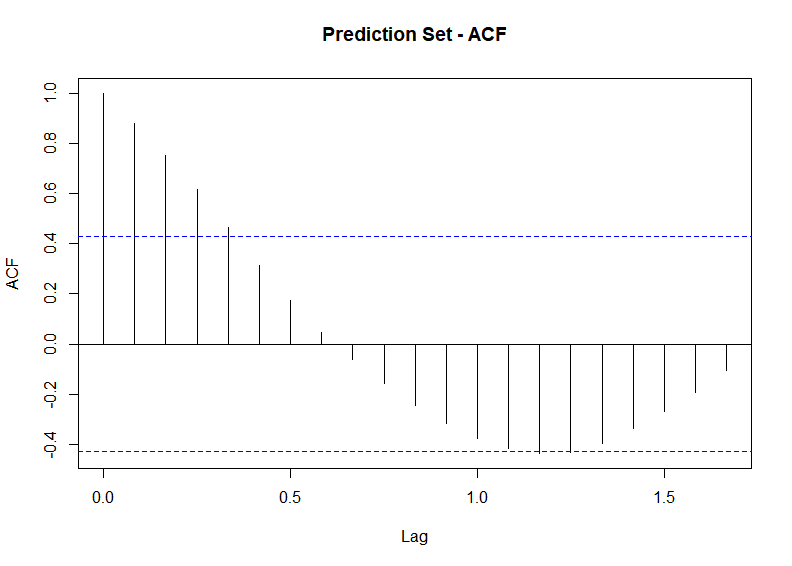
\includegraphics[width=5.20833in,height=5.20833in]{03_visuals/pred_acf.png}

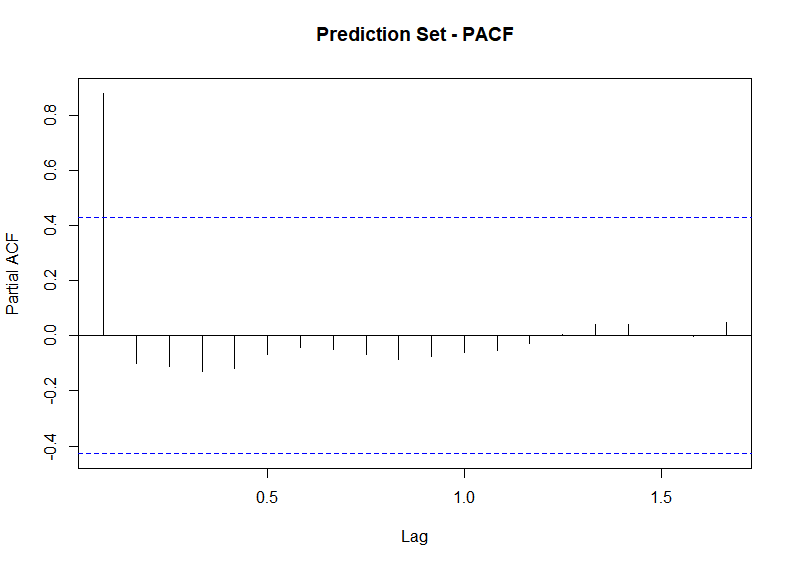
\includegraphics[width=5.20833in,height=5.20833in]{03_visuals/pred_pacf.png}

We then also created ACF and PACFs based on the logged differences.

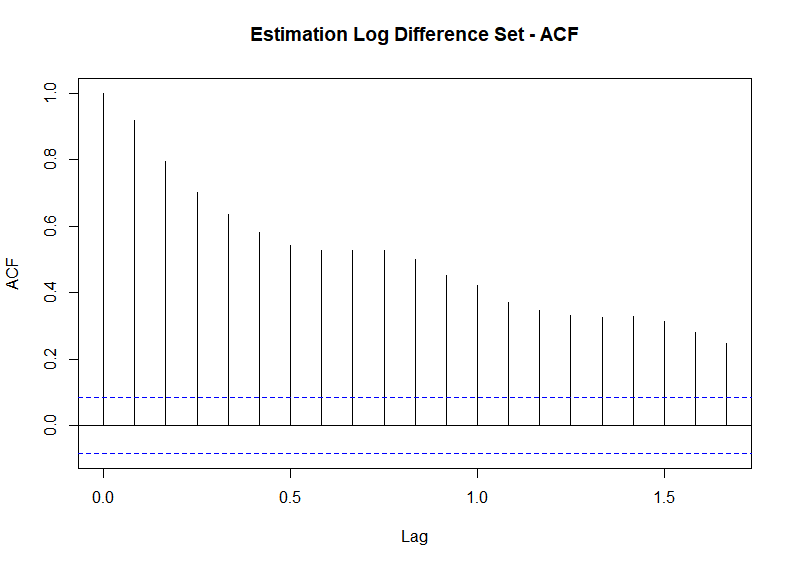
\includegraphics[width=5.20833in,height=5.20833in]{03_visuals/ld_est_acf.png}

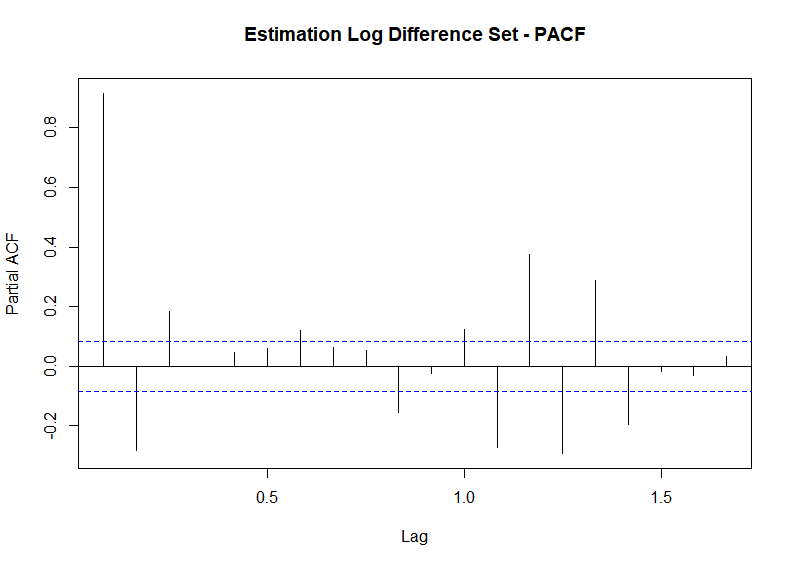
\includegraphics[width=5.20833in,height=5.20833in]{03_visuals/ld_est_pacf.png}

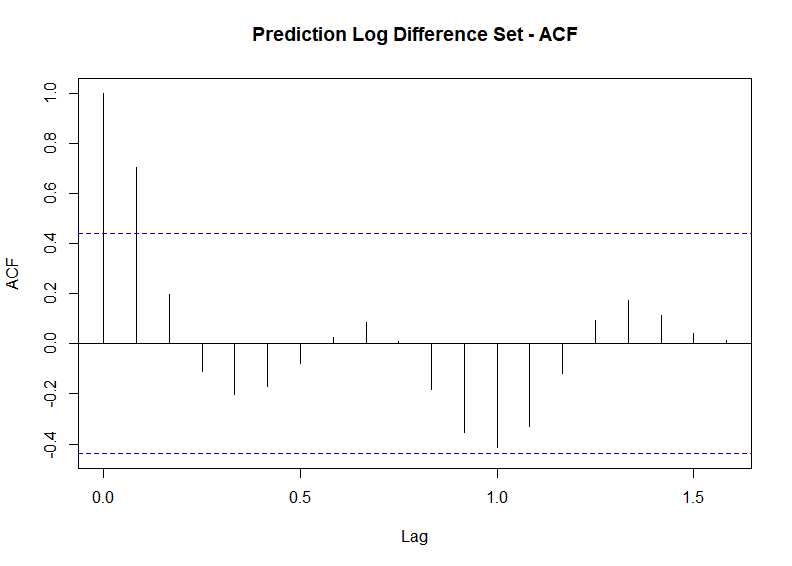
\includegraphics[width=5.20833in,height=5.20833in]{03_visuals/ld_pred_acf.png}

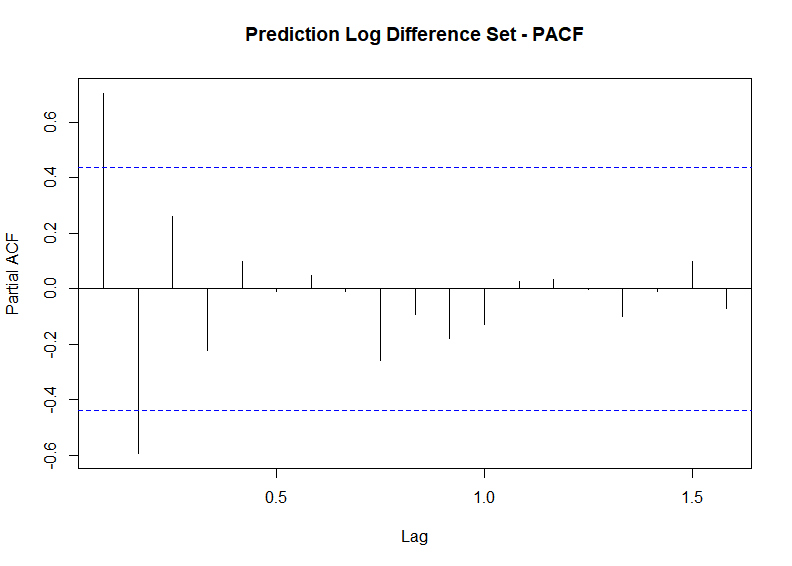
\includegraphics[width=5.20833in,height=5.20833in]{03_visuals/ld_pred_pacf.png}

\end{document}
